\documentclass{book}

\usepackage{amssymb}
\usepackage{amsmath}
\usepackage{amsthm}
\usepackage{arydshln}
\usepackage{calc}
\usepackage{cancel}
\usepackage{caption}
\usepackage{cite}
\usepackage{color}
\usepackage{enumitem}
\usepackage{esint}
\usepackage{etoolbox}
\usepackage{float}
\usepackage{framed}
\usepackage{fullpage}
\usepackage{gensymb}
\usepackage[margin=1in]{geometry}
\usepackage{graphicx}
\usepackage{listings}
\usepackage{multirow}
\usepackage{subfiles}
\usepackage{rsfso}
\usepackage{tikz}
\usepackage{tikz-3dplot}
\usepackage{ushort}
\usepackage{wrapfig}
\usepackage{xcolor}
\usepackage{soul}
\usepackage{epstopdf}
\usepackage{pgfplots}

% pdf versions
\pdfoptionpdfminorversion=7

% handle page stretching
\raggedbottom

% Graphics file location
\graphicspath{{Graphics/}{../Graphics/}}

% Use for drawings
\usetikzlibrary{angles,arrows,calc,decorations,intersections,patterns,positioning,quotes,shapes}
\usetikzlibrary{shapes.geometric}
\usetikzlibrary{decorations.pathreplacing}
\newcommand{\midarrow}{\tikz \draw[-latex] (0,0) -- +(.1,0);}

% Tikz commands for drawing block diagrams, etc...
\tikzset{%
	block/.style    = {draw, rectangle, minimum height = 2em, minimum width = 2em},
	sum/.style      = {draw, circle}, % Adder
	input/.style    = {fill=white, rectangle}, % Input
	output/.style   = {fill=white, rectangle}, % Output
	waypoint/.style   = {coordinate}, % Output
}

\tikzset{%
	startstop/.style= {draw, rectangle, rounded corners, minimum width=2cm, minimum height=1cm,text centered},
	inout/.style    = {draw, trapezium, trapezium left angle=70, trapezium right angle=110, minimum width=2cm, minimum height=1cm, text centered},
	process/.style  = {draw, rectangle, minimum width=2cm, minimum height=1cm, text centered},
	decision/.style = {draw, diamond, minimum width=1.5cm, minimum height=1cm, text centered, diamond, aspect=2},
	arrow/.style    = {thick,-latex,>=stealth},		
}

\tikzset{
	saveuse path/.code 2 args={
		\pgfkeysalso{#1/.style={insert path={#2}}}%
		\global\expandafter\let\csname pgfk@\pgfkeyscurrentpath/.@cmd\expandafter\endcsname
		% not optimal as it is now global through out the document
		\csname pgfk@\pgfkeyscurrentpath/.@cmd\endcsname
		\pgfkeysalso{#1}},
	/pgf/math set seed/.code=\pgfmathsetseed{#1}}

% Define Laplace, Fourier transform symbols
\newcommand{\LT}{\mathcal{L}}
\newcommand{\FT}{\mathcal{F}}

% Define adjugate function
\newcommand{\adj}{\text{adj}}

% Define rank function
\newcommand{\rank}{\text{rank}}

% commands to speed up writing j\omega and s-plane
\newcommand{\jw}{j\omega}
\newcommand{\spl}{s\textrm{-plane}}
\newcommand{\wt}{\omega t}
\newcommand{\Lm}{\textrm{Lm }}
% Clean up overline/underline for math mode
\def\obar#1{\bar{#1}}
\def\ubar#1{\ushort{#1}}

\newcommand{\exmp}{\subsubsection*{Example}}
\newcommand{\nib}{\noindent$ \bullet\ $}


\begin{document}
\chapter*{Lecture 16}
Last lecture:
\begin{itemize}
	\item Loop Shaping: Give our closed-loop system good performance by giving the Bod plot of our open-loop transfer function $ G_cG_p $ a good shape.
	\item The closed-loop system will reject disturbances and have low steady-state error if $ G_cG_p $ has large magnitude for low frequencies.
	\item The closed-loop system will attenuate noise if $ G_cG_p $ has small magnitude for high frequencies.
	\item The closed-loop system will be stable and robust if the slope of $ \Lm G_cG_p $ is $ -20 $dB/decade at or near the 0dB crossover.
	\begin{center}
		\begin{tikzpicture}[scale=1.25]
		\draw (0,3.5) node[left] {$\Lm M$} |- (5,0) node[below left] {$ \omega $};
		
		\draw[dashed] (0,1.5) node[left] {0dB} -| (2.5,0) node[below] {$ \omega_c $};
		\draw[thick] (0,3)-- (0.78125,2.375) ..controls (1.5625,1.75) .. (2.5,1.5) ..controls (3.4375,1.25) .. (4.21875,.625) -- (5,0);
		\node at (0.78125,2.375) {\begin{tikzpicture}[scale=0.5] \draw[dashed,rotate=-40] (0,0) ellipse (2.5 and 0.5); \end{tikzpicture}};
		\node at (2.5,1.5) {\begin{tikzpicture}[scale=0.5] \draw[dashed,rotate=-15] (0,0) ellipse (2 and 0.5);\end{tikzpicture}};
		\node at (4.21875,.625) {\begin{tikzpicture}[scale=0.5] \draw[dashed,rotate=-40] (0,0) ellipse (2.5 and 0.5); \end{tikzpicture}};
		
		\draw[-latex] (1.5,3.25) node[right,align=left] {Good disturbance rejection\\ \& low steady-state error.} -- (1,2.5625);
		\draw[-latex] (3,2.375) node[right,align=left] {Good stability margins.} -- (2.6875,1.6875);
		\draw[-latex] (4.375,1.5) node[right,align=left] {Good noise\\attenuation.} -- (4.1875,1);
		\end{tikzpicture}
	\end{center}	
	\item If we want our closed-loop system to behave like a second-order system,
	\[ \frac{\omega_n^2}{s^2+2\zeta\omega_ns + \omega_n^2} \]
	then  our open-loop transfer function should look something like
	\[ G_cG_p = \frac{\frac{\omega_n}{2\zeta}}{s\left(\frac{s}{2\zeta\omega_n}+1\right)} \]
	\begin{center}
		\begin{tikzpicture}
		\draw (0,0) node[left] {0dB} -- (4,0);
		\draw (0,0.5) -- (2,-0.5) -- ( 3,-1.5);
		\draw [decorate,decoration={brace,amplitude=10pt}, yshift=-4pt] (4.25,-2) -- (-0.75,-2) node [below,black,midway,yshift=-10pt,align=center] {$ \zeta>\frac{1}{2} $};
		\node[below] at (1,0) {$ \frac{\omega_n}{2\zeta} $};
		\draw[dashed] (2,0) node[above] {$ 2\zeta\omega_n $} -- (2,-0.5);
		\node at (1,0) {$ * $};
		
		\draw[xshift=5.5cm] (0,0) node[left] {0dB} -- (4,0);
		\draw[xshift=5.5cm] (0,1) -- (2,0) -- (3.5,-1.5);
		\draw [decorate,decoration={brace,amplitude=10pt}, yshift=-4pt] (9.75,-2) -- (4.75,-2) node [below,black,midway,yshift=-10pt,align=center] {$ \zeta=\frac{1}{2} $};
		\node[above right] at (7.5,0) {$ 2\zeta\omega_n = \frac{\omega_n}{2\zeta} $};
		\node at (7.5,0) {$ * $};
		
		\draw[xshift=11cm] (0,0) node[left] {0dB} -- (4,0);
		\draw[xshift=11cm] (0,1.5) -- (2,0.5) -- (3.75,-1.5);
		\draw [decorate,decoration={brace,amplitude=10pt}, yshift=-4pt] (15.25,-2) -- (10.25,-2) node [below,black,midway,yshift=-10pt,align=center] {$ \zeta<\frac{1}{2} $};\node[below] at (1,0) {$ \frac{\omega_n}{2\zeta} $};
		\draw[dashed] (13,0.5) -- (13,0) node[below] {$ 2\zeta\omega_n $};
		\node[above right] at (13.5,0) {$ \frac{\omega_n}{2\zeta} $};
		\node at (13.5,0) {$ * $};
		\end{tikzpicture}
	\end{center}
\end{itemize}

This lecture: Controller design steps.

First, let's do some examples for what we learned last lecture.

\exmp
What do we want $ G_cG_p $ to look like if we want and overshoot percent and peak time such that $ \zeta = \sqrt{2.5} $ and $ \omega_n = 2\sqrt{2.5} $?
\[ G_cG_p = \frac{\frac{2\sqrt{2.5}}{2(\sqrt{2.5})}}{s\left(\frac{s}{2(\sqrt{2.5})(2\sqrt{2.5})}+1\right)} \]
\[ G_cG_p = \frac{1}{s\left(\frac{s}{10}+1\right)} \]

\exmp
What do we want $ G_cG_p $ to look like if we want and overshoot percent and peak time such that $ \zeta = \frac{1}{2}\sqrt{10} $ and $ \omega_n = 40\sqrt{10} $?
\[ G_cG_p = \frac{\frac{40\sqrt{10}}{2(\frac{1}{2}\sqrt{10})}}{s\left(\frac{s}{2(\frac{1}{2}\sqrt{10})(40\sqrt{10})}+1\right)} \]
\[ G_cG_p = \frac{40}{s\left(\frac{s}{400}+1\right)} \]

\subsection*{Controller Design Steps}
\begin{enumerate}
	\item Transient requirements $ \Longrightarrow $ $ \omega_n$, $\zeta $
	\item Desired open-loop transfer function:
	\[ G_cG_p = OLTF = \frac{\frac{\omega_n}{2\zeta}}{s\left(\frac{s}{2\zeta\omega_n}+1\right)} \]
	\item $ G_c =$ what we have to add to $ G_p $ in order to make $ G_cG_p $ look like OLTF (look like $ \frac{{\omega_n}/{2\zeta}}{s\left(\frac{s}{2\zeta\omega_n}+1\right)} $)
\end{enumerate}
This seems easy when $ G_p $ is really simple.

\subsection*{What do we do if $ G_p $ is more complicated and/or has extra poles/zeros?}
\begin{itemize}
	\item Previously, we said our system would behave like a 2nd order system if extra poles/zeros are far enough left. % For Root Locus design, 
	\item For loop shaping, our closed-loop system will behave like a second-order system if $ G_cG_p $ has the right shape near the 0dB crossover
	\item Note: ``near'' means ``within about 1 decade'' ($ \approx \pm 1 $ decade) or dictated by $ \zeta $ and $ \omega_n $.
	\begin{center}
		\begin{tikzpicture}
		\draw (0,0) node[left] {0dB} -- (4,0);
		\draw (0,1) -- (0.333,1) -- (0.667,0.667) -- (1,0.667) -- (1.333,0.333) -- (2.667,-0.333) -- (3,-1) -- (3.5,-1.167) -- (4,-1.5);
		
		\draw[xshift=6cm] (0,0) node[left] {0dB} -- (4,0);
		\draw[xshift=6cm] (0,1) -- (2.667,-0.333) -- (4,-1.5);	
		
		\node at (4.625,0) {\Large$ \approx $};
		\end{tikzpicture}
	\end{center}
	\begin{itemize}
		\item Still large at low freq. $ \rightarrow $ rejects disturbances, low $ e_{ss} $.
		\item Still small at high freq. $ \rightarrow $ attenuates noise
		\item Similar shape near 0dB $ \rightarrow $ stable, robust, $ \sim $second order
	\end{itemize}
\end{itemize}

\clearpage
\exmp
Velocity control of a trolley (mass $ m=1 $kg) moving on a straight path, with actuator force $ u $ as the input $ u $ and velocity $ y $ as the output. For a step input, we want $ OS\% < 20\% $, $ t_s \leq 12 $.
\begin{center}
	\begin{tikzpicture}
	\node[draw, rectangle, minimum height = 2.5em, minimum width = 4em] (M) {$ m $};
	\draw[thick,-latex] ([xshift=-1cm]M.west) node[left] {$ u $} -- (M.west);
	\draw[-latex] (M.north) |- ([xshift=0.75cm,yshift=0.5cm]M.north) node[right] {$ y $} ;
	\end{tikzpicture}
	
	\vspace{1em}
	
	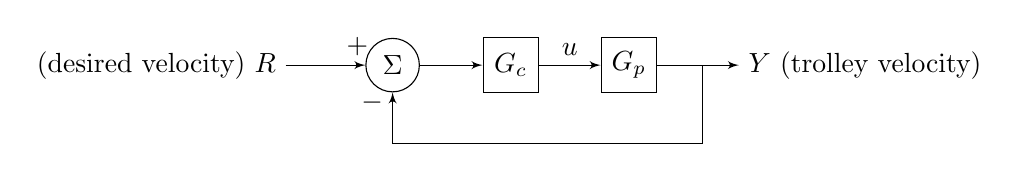
\begin{tikzpicture}[node distance=1.50cm,auto,>=latex']
	\node [input] (r) {(desired velocity) $R$};
	\node [sum] (sumr) [right of=r,node distance=3cm] {$\Sigma$};
	\node [block] (gc) [right of=sumr] {$ G_c $};
	\node [block] (gp) [right of=gc] {$ G_p $};
	\node [output] (y) [right of=gp,node distance=3cm]{$Y$ (trolley velocity)};
	\node [waypoint] (wp) [below of=gp,node distance=1cm] {};
	
	\draw[->] (r) -- node[pos=0.9] {$+$} (sumr);
	\draw[->] (sumr) -- (gc);
	\draw[->] (gc) -- node[above] {$ u $} (gp);
	\draw[->] (gp) -- (y);
	\draw[->] ($ (gp)!0.3125!(y) $) |- (wp)-| node[pos=0.9] {$-$} (sumr);
	\end{tikzpicture}
\end{center}
\[ G_p:\quad F=ma \quad\Rightarrow\quad u(t) = m\dot{y}(t) \]
\[ \Rightarrow U(s)=msY(s) \quad\Rightarrow\quad \frac{Y}{U} = G_p = \frac{1}{ms} = \frac{1}{s} \]	
\[ OS\% < 20\% \quad\Rightarrow\quad \zeta \geq 0.6 \]
\[ t_s \leq 12 \quad\Rightarrow\quad \omega_n \geq 0.55 \]
Let's pick $ \zeta =0.6 $ and $ \omega_n = 0.6 $. Then, our desired $ G_cG_p $ is
\[ \text{Desired } G_cG_p = \frac{\frac{\omega_n}{2\zeta}}{s\left(\frac{s}{2\zeta\omega_n}+1\right)}  = \frac{\frac{0.6}{2\cdot0.6}}{s\left(\frac{s}{2\cdot0.6\cdot0.6}+1\right)}= \frac{0.5}{s\left(\frac{s}{0.72}+1\right)} \]
\begin{center}
	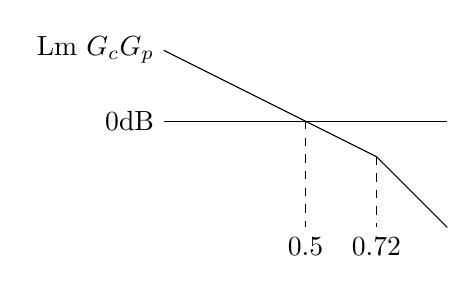
\begin{tikzpicture}[scale=0.9]
	\draw (0,0) node[left] {0dB} -- (4,0);
	\draw (0,1) node[left] {Lm $ G_cG_p $} -- (3,-0.5) -- (4,-1.5);
	\draw[dashed] (2,0) -- (2,-1.5) node[below] {$ 0.5 $};
	\draw[dashed] (3,-0.5) -- (3,-1.5) node[below] {$ 0.72 $};
	\end{tikzpicture}
\end{center}
Knowing that $ G_p=1/s $, we can quickly identify what we want for $ G_c $ from the desired $ G_cG_p $:
\[ \text{Desired } G_cG_p = \underbrace{\frac{1}{s}}_{G_p} \cdot \underbrace{\frac{0.5}{\frac{s}{0.72}+1}}_{G_c} \quad\Rightarrow\quad G_c = \frac{0.5}{\frac{s}{0.72}+1} \]

\begin{center}
\end{center}

\begin{minipage}{0.49\textwidth}
	However, let's explore the design process in greater detail. Before designing $ G_c $, what does the plant log magnitude look like?\vspace{1em}
	
	This meets some but not all of our requirements:
	\begin{itemize}
		\item Big at low frequencies
		\item Small at high frequencies
		\item Robust stability and performance
	\end{itemize}	
	
	But, it does not have a second-order shape, so we will not meet our transient requirements. What is missing? We need a corner at $ \omega = 0.72 $. So, we add a pole to $ G_c $:
	\[ \frac{1}{\frac{s}{0.72}+1} \]
	
	Next, we need the low-frequency asymptote to cross 0dB at $ \omega=0.5 $.
	\begin{itemize}
		\item We use a gain to shift the Lm plot.
		\item The low-frequency asymptote is currently $ \sim6 $dB at $ \omega=0.5 $, so we need $ G_c $ to provide $ -6$dB of gain.
		\[ \Lm(K) = 20\log_{10}(K) = -6 \]
		\[ \log_{10}(K) = -0.3 \quad\rightarrow\quad K = 10^{-0.3} = 0.5 \]	 
	\end{itemize}
	
	So,
	\[ \boxed{G_c = \frac{0.5}{\frac{s}{0.72}+1}} \]
\end{minipage}
\begin{minipage}{0.49\textwidth}
	\centering
	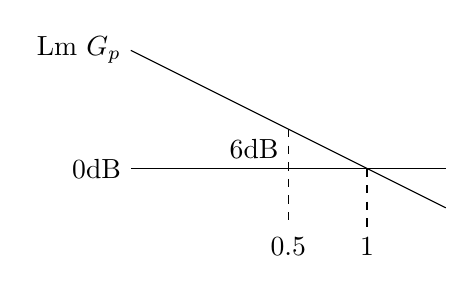
\begin{tikzpicture}
	\draw (0,0) node[left] {0dB} -- (4,0);
	\draw (0,1.5) node[left] {Lm $ G_p $} -- (3,0) -- (4,-0.5);
	\draw[dashed] (2,0.5) -- node[left] {6dB} (2,0) -- (2,-0.75) node[below] {$ 0.5 $};
	\draw[dashed] (3,0) -- (3,-0.75) node[below] {$ 1 $};
	\end{tikzpicture}\\
	
	\vspace{6em}
	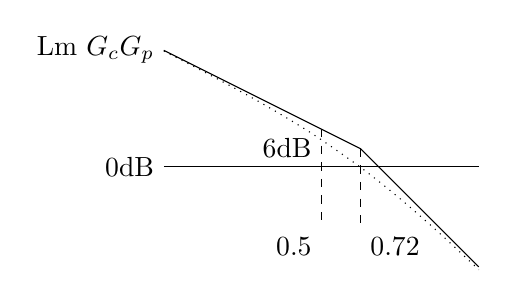
\begin{tikzpicture}
		\draw[yshift=0.024776998cm] (0,0) node[left] {0dB} -- (4,0);
		\draw (0,1.5) node[left] {Lm $ G_cG_p $} -- (2.5,0.25) -- (4,-1.25);
		\draw[dashed] (2,0.5) -- node[left] {6dB} (2,0.024776998cm) -- (2,-0.75) node[below left] {$ 0.5 $};
		\draw[dashed] (2.5,0.25) -- (2.5,-0.75) node[below right] {$ 0.72 $};
		\draw[smooth,dotted] plot coordinates {(0,1.491) (0.625,1.166) (1.25,0.8237) (1.875,0.4467) (2.5,0.01239) (3,-0.3849) (3.5,-0.8217) (4,-1.286)};
	\end{tikzpicture}\\
	
	\vspace{2em}
	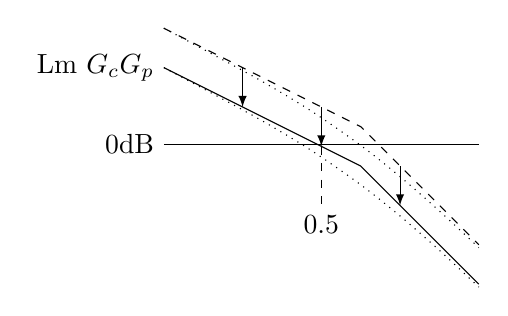
\begin{tikzpicture}
		\draw[yshift=0.024776998cm] (0,0) node[left] {0dB} -- (4,0);
		\draw[dashed] (0,1.5) -- (2.5,0.25) -- (4,-1.25);
		\draw (0,1) node[left] {Lm $ G_cG_p $} -- (2.5,-0.25) -- (4,-1.75);
		\draw[dashed] (2,0) -- (2,-0.75) node[below] {$ 0.5 $};
		\draw[smooth,dotted] plot coordinates {(0,1.5) (0.625,1.166) (1.25,0.8237) (1.875,0.4467) (2.5,0.0124) (3,-0.3849) (3.5,-0.8217) (4,-1.287)};
		\draw[smooth,dotted,yshift=-0.5cm] plot coordinates {(0,1.5) (0.625,1.166) (1.25,0.8237) (1.875,0.4467) (2.5,0.0124) (3,-0.3849) (3.5,-0.8217) (4,-1.287)};
		\draw[-latex] (1,1) -- (1,0.5);
		\draw[-latex] (2,0.5) -- (2,0);
		\draw[-latex] (3,-0.25) -- (3,-0.75);
	\end{tikzpicture}
	
	\vspace{4em}	
\end{minipage}
\clearpage
\exmp
Consider the above example again, except this the output $ y(t) $ is the position rather than the velocity.
\begin{center}
	\begin{tikzpicture}
	\node[draw, rectangle, minimum height = 2.5em, minimum width = 4em] (M) {$ m $};
	\draw[thick,-latex] ([xshift=-1cm]M.west) node[left] {$ u $} -- (M.west);
	\draw[-latex] (M.north) |- ([xshift=0.75cm,yshift=0.5cm]M.north) node[right] {$ y $} ;
	\end{tikzpicture}
	
	\vspace{1em}
	
	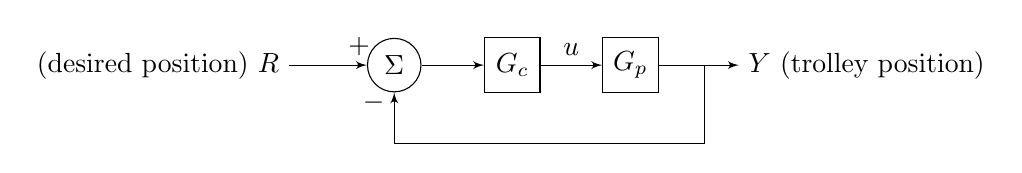
\begin{tikzpicture}[node distance=1.50cm,auto,>=latex']
	\node [input] (r) {(desired position) $R$};
	\node [sum] (sumr) [right of=r,node distance=3cm] {$\Sigma$};
	\node [block] (gc) [right of=sumr] {$ G_c $};
	\node [block] (gp) [right of=gc] {$ G_p $};
	\node [output] (y) [right of=gp,node distance=3cm]{$Y$ (trolley position)};
	\node [waypoint] (wp) [below of=gp,node distance=1cm] {};
	
	\draw[->] (r) -- node[pos=0.9] {$+$} (sumr);
	\draw[->] (sumr) -- (gc);
	\draw[->] (gc) -- node[above] {$ u $} (gp);
	\draw[->] (gp) -- (y);
	\draw[->] ($ (gp)!0.3125!(y) $) |- (wp)-| node[pos=0.9] {$-$} (sumr);
	\end{tikzpicture}
\end{center}
Then,
\[ G_p:\quad F=ma \quad\Rightarrow\quad u(t) = m\ddot{y}(t) \]
\[ \Rightarrow U(s)=ms^2Y(s) \quad\Rightarrow\quad \frac{Y}{U} = G_p = \frac{1}{ms^2} = \frac{1}{s^2} \]
For this example, we will use $ \zeta=0.6 $ and $ \omega=2 $, so the desired $ G_cG_p $ will be
\[\frac{\frac{\omega_n}{2\zeta}}{s\left(\frac{s}{2\zeta\omega_n}+1\right)}  = \text{Desired } G_cG_p = \frac{\frac{5}{3}}{s\left(\frac{s}{2.4}+1\right)} \]
This time, we have an extra integrator in $ G_p $, so it will be more challenging to design $ G_c $. $ 1/s $ is an unstable pole, so we cannot simply cancel the extra integrator with a zero at $ s=0 $ (we would lose internal stability). In this example we will explore how to design $ G_c $ for the more complicated plant.\\

\noindent Before designing $ G_c $, what does the open-loop log magnitude look like?
\begin{center}
	\begin{tikzpicture}[yscale=0.8]
	\draw (0,0) node[left] {0dB} -- (4,0);
	\draw (0.5,1.5)  -- (2,0) -- (3.5,-1.5);
	\node[left] at (0,1.5) {Lm $ G_p $};
	\draw[dashed] (2,0) -- (2,-1.5) node[below] {$ 1 $};
	\end{tikzpicture}
\end{center}
This meets two of our requirements:
\begin{itemize}
	\item Big at low frequencies
	\item Small at high frequencies
\end{itemize}
However, it does not have $ -20 $dB/decade of slope near the 0dB crossover, so:
\begin{itemize}
	\item Not stable and not robust
	\item No 2nd-order shape
\end{itemize}
What we really want is a shape like this:
\begin{center}
	\begin{tikzpicture}[xscale=1.25]
	\draw (0,0) node[left] {0dB} -- (4,0);
	\draw (0,1) node[left] {Desired Lm $ G_cG_p $} -- (3,-0.5) -- (4,-1.5);
	\draw[dashed,align=center] (2,0) -- (2,-1.5) node[below] {$ \frac{\omega_n}{2\zeta}$\\$=1.67$};
	\draw[dashed,align=center] (3,-0.5) -- (3,-1.5) node[below] {$2\zeta\omega_n$\\ $=2.4 $};
	\end{tikzpicture}
\end{center}
How can we get our desired shape near the crossover?
\begin{itemize}
	\item Add a zero and a pole
	\begin{itemize}
		\item We want the pole at $ \omega=2\zeta\omega_n=2.4 $
		\item We must place the zero before $ \omega=\frac{\omega_n}{2\zeta}=1.67 $. We will say the zero is at $ \omega=\omega_1 $.
	\end{itemize}
	\item Add a gain $ K $ to get the 0dB crossover we want
	\item Remember: we cannot add a zero at $ s=0 $, canceling the $ s=0 $ pole. This would create a ``hidden instability''.
\end{itemize}
So, our controller will have the form
\[ G_c = K\cdot\frac{\frac{s}{\omega_1}+1}{\frac{s}{2.4}+1} \]
We want $ \omega_1 $ at least 1 decade away from the 0dB crossover. Let's pick $ \omega_1=0.1 $. Now, let's find $ K $:
\begin{itemize}
	\item The $ -20 $dB/decade asymptote should be 0dB at $ \omega = \frac{\omega_n}{2\zeta}=1.67 $
	\item If $ G_c = \frac{\frac{s}{0.1}+1}{\frac{s}{2.4}+1} $ then the magnitude of $ G_cG_p $ will be 14dB at $ \omega=1.67 $.
	\[ \Lm G_cG_p (1.67) = 20\log_{10}\left(  \frac{\sqrt{\left(\frac{1.67^2}{0.1^2}\right)+1}}{1.67^2\sqrt{\left(\frac{1.67^2}{2.4^2}\right)+1}}  \right) = 14\textrm{dB}\]
	
	% (The -20dB/decade asymptote is at about 15.5dB, but the actual value is lower due to its proximity to the 2.4 rad/s pole.)
	
%	To estimate this from the asymptotes, we simply use $ \Delta y = \textrm{slope} \times \Delta x $:
%	\begin{itemize}
%		\item We know that we start at 40dB at $ \omega = 0.1 = 10^{-1} $, and have $ -20 $dB/dec slope. 
%		\item The change in $ x $ from $ \omega=0.1 $ to $ \omega = 1.67 $ is $ \log_{10}(1.67) - \log_{10} (0.1) = 0.223 - (-1) = 1.223 $ decades. 
%		\item So, the change in LM from $ \omega=0.1 $ to $ \omega = 1.67 $ is $ -20 \textrm{ db/dec} \times 1.223 \textrm{ dec} = -24.5$dB.
%		\item So, the \textit{approximate} LM at $ \omega=1.67 $ is 40db $ - 24.5 $dB$ =15.5 $dB. 
%		\item Again, the \textit{true} magnitude at $ \omega=1.67 $ is slightly lower, due to the change in slope at $ \omega=2.4 $.
%	\end{itemize}
	\begin{center}
		\begin{tikzpicture}[scale=1.125,xscale=1.5,yscale=0.025]
		\draw (-2,0) node[left] {0dB} -- (2,0);
		\draw (-2,80) -- (2,-80) node[right] {$ G_p $};
		\draw[dashed] (-2,80) -- (-1,40) -- (0.38,12.4) -- (2,-52.4) node[right] {$ G_cG_p $};
		\draw[dotted] (-2,40) node[left] {40dB} -- (-1,40) -- (-1,-80) node[below] {$0.1 $};
		\draw[dotted] (0.2218,15.5) -- (0.2218,-95) node[below] {$1.67$};
		\draw[dotted] (0.3802,12.4) -- (0.3802,-80) node[below] {$2.4 $};
		\draw (0.75,27.75) node[right]{14dB} -- (0.2218+0.08,7.75);
		
		
		\draw[dotted] (-2,20) node[left] {20dB} -- (0,20) -- (0,-80) node[below] {$1 $};
		
		\draw [decorate,decoration={brace,amplitude=4pt}, yshift=-4pt] (0.2218,15.5) -- (0.2218,0);
		
		\end{tikzpicture}
	\end{center}
	\item So, add a gain that will shift the log magnitude by $ -14 $dB
	\[ \Lm(K) = 20\log_{10}(K) = -14 \]
	\[ \log_{10}(K) = -0.7 \quad\rightarrow\quad K = 10^{-0.7} \approx 0.2 \]
\end{itemize}
Therefore,
\[ \boxed{G_c = \frac{0.2\left(\frac{s}{0.1}+1\right)}{\frac{s}{2.4}+1}} \]
\clearpage

\exmp
\begin{center}
	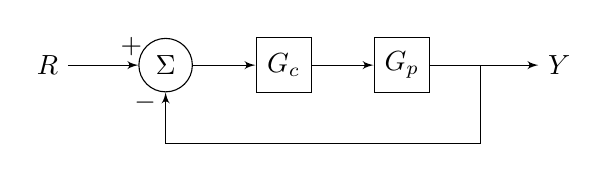
\begin{tikzpicture}[node distance=1.50cm,auto,>=latex']
	\node [input] (r) {$R$};
	\node [sum] (sumr) [right of=r] {$\Sigma$};
	\node [block] (gc) [right of=sumr] {$ G_c $};
	\node [block] (gp) [right of=gc] {$ G_p $};
	\node [output] (y) [right of=gp,node distance=2cm]{$Y$};
	\node [waypoint] (wp) [below of=gp,node distance=1cm] {};
	
	\draw[->] (r) -- node[pos=0.9] {$+$} (sumr);
	\draw[->] (sumr) -- (gc);
	\draw[->] (gc) --  (gp);
	\draw[->] (gp) -- (y);
	\draw[->] ($ (gp)!0.5!(y) $) |- (wp)-| node[pos=0.9] {$-$} (sumr);
	\end{tikzpicture}
\end{center}
\[ G_p = \frac{1}{\frac{s}{3}+1} \]
Find $ G_c $ such that:
\begin{itemize}
	\item $ t_s\leq 3 $s
	\item $ OS\% \leq 5\% $
	\item $ e_{ss}\leq 5\% $
\end{itemize}
What we have:
\begin{center}
	\begin{tikzpicture}[scale=1.5,yscale=0.025]
	\draw (-2,40) node[below left] {Lm $ G_p $} |- (2,-40) node[below left] {$ \omega$};
	\draw (-2,0) node[left] {0dB} -- (0.4771,0) -- (2,-30.4576);
	% \draw[dashed] (-2,80) -- (-1,40) -- (0.38,12.4) -- (2,-52.4);
	\draw[dotted] (0.4771,0) -- (0.4771,-40) node[below] {$\omega=3 $};
	% \draw[dotted] (0.2218,15.5) -- (0.2218,-80) node[below left] {$1.67$};
	% \draw[dotted] (0.3802,12.4) -- (0.3802,-80) node[below right] {$2.4 $};
	% \draw[->] (0.75,27.75) node[right]{15.5dB} -- (0.2218,7.75);
	\end{tikzpicture}
\end{center}
What we want:
\begin{center}
	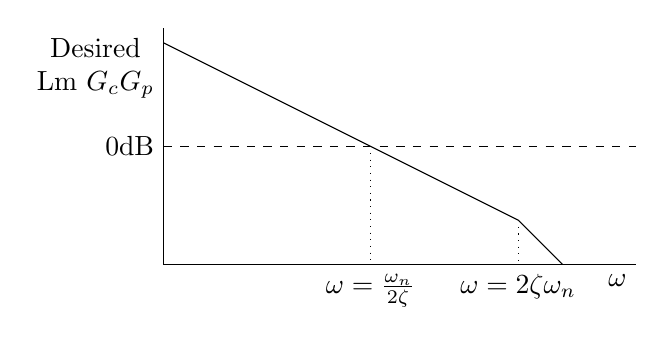
\begin{tikzpicture}[scale=1.5,yscale=0.025]
	\draw (-2,40) node[below left,align=center] {Desired\\Lm $ G_cG_p $} |- (2,-40) node[below left] {$ \omega$};
	\draw[dashed] (-2,0) node[left] {0dB} -- (2,0);
	\draw (-2,35)  -- (1,-25) -- (1.375,-40);
	% \draw[dashed] (-2,80) -- (-1,40) -- (0.38,12.4) -- (2,-52.4);
	\draw[dotted] (-0.25,0) -- (-0.25,-40) node[below] {$\omega=\frac{\omega_n}{2\zeta} $};
	\draw[dotted] (1,-25) -- (1,-40) node[below] {$\omega={2\zeta\omega_n} $};
	% \draw[dotted] (0.2218,15.5) -- (0.2218,-80) node[below left] {$1.67$};
	% \draw[dotted] (0.3802,12.4) -- (0.3802,-80) node[below right] {$2.4 $};
	% \draw[->] (0.75,27.75) node[right]{15.5dB} -- (0.2218,7.75);
	\end{tikzpicture}
\end{center}
What should we do?
\begin{itemize}
	\item It depends on if the pole of $ G_p $ is in a convenient place.
	\item Let's look at the transient requirements:
	\begin{itemize}
		\item $ OS\% \leq 5\% $: $ \zeta \geq 0.69 $. Let's use $ \zeta=0.7 $.
		\item $ t_s = \frac{4}{\omega_n\zeta} \leq 3 $: $ \frac{4}{3} \leq \omega_n\zeta \ \rightarrow\ 2\zeta\omega_n \geq 2 \frac{2}{3} $
	\end{itemize}
	\item Therefore, the pole is at a convenient place ($ 2\zeta\omega_n = 3 \geq 2 \frac{2}{3} $)
	\item So, we will give $ G_c $ a pole at the origin and a gain that will cause a good 0dB crossover.
	\[ 2\zeta\omega_n = 3 \ \Rightarrow\ \omega_n = \frac{3}{2\zeta} \]
	\[ \text{crossover: } \frac{\omega_n}{2\zeta} = \frac{\frac{3}{2\zeta}}{2\zeta} = \frac{3}{4\zeta^2} \approx 1.53  \]
	Then,
	\[ (G_cG_p)_{desired} = \frac{1.53}{s(\frac{s}{3}+1)},\ G_p = \frac{1}{\frac{s}{3}+1} \quad\Rightarrow\quad G_c = \frac{1.53}{s}  \]
	\item Because of the integrator in $ G_c $, $ e_{ss}=0 $.
\end{itemize}

\exmp
$ G_p $ is a second-order system with $ \omega_n=\frac{3}{2} $ and $ \zeta=\frac{2}{3} $.
\[ G_p = \frac{1}{\frac{1}{\omega_n^2}s^2+\frac{2\zeta}{\omega_n}s+1} = \frac{1}{\frac{4}{9}s^2+\frac{8}{9}s+1} \]
Find $ G_c $ such that:
\begin{itemize}
	\item $ t_s\leq 3 $s
	\item $ OS\% \leq 5\% $
	\item $ e_{ss}\leq 5\% $
\end{itemize}
What we have:
\begin{center}
	\begin{tikzpicture}[scale=1.5,yscale=0.025]
	\draw (-2,40) node[below left] {Lm $ G_p $} |- (2,-40) node[below left] {$ \omega$};
	\draw (-2,0) node[left] {0dB} -- (0.1761,0) -- (1.1761,-40);
	\draw[dotted] (0.1761,0) -- (0.1761,-40) node[below] {$\omega=\frac{3}{2} $};
	\draw[->] (1,7.75) node[above]{-40dB/dec} -- (0.6716,-20);
	\end{tikzpicture}
\end{center}
What we want:
\begin{center}
	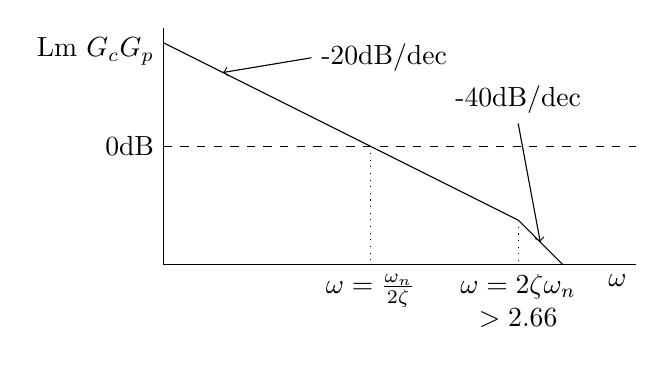
\begin{tikzpicture}[scale=1.5,yscale=0.025]
	\draw (-2,40) node[below left] {Lm $ G_cG_p $} |- (2,-40) node[below left] {$ \omega$};
	\draw[dashed] (-2,0) node[left] {0dB} -- (2,0);
	\draw (-2,35)  -- (1,-25) -- (1.375,-40);
	% \draw[dashed] (-2,80) -- (-1,40) -- (0.38,12.4) -- (2,-52.4);
	\draw[dotted] (-0.25,0) -- (-0.25,-40) node[below] {$\omega=\frac{\omega_n}{2\zeta} $};
	\draw[dotted,align=center] (1,-25) -- (1,-40) node[below] {$\omega={2\zeta\omega_n} $\\$ >2.66 $};
	\draw[->] (1,7.75) node[above]{-40dB/dec} -- (1.1875,-32.5);
	\draw[->] (-0.75,30) node[right]{-20dB/dec} -- (-1.5,25);
	\end{tikzpicture}
\end{center}
\begin{itemize}
	\item We know from the previous example that $ 2\zeta\omega_n \geq 2 \frac{2}{3} $
	\item What do we do?
	\begin{itemize}
		\item Cancel the poles of $ G_p $
		\item Design a controller that undoes the dynamics of the plant and replaces them with better dynamics
		\item If we want to give the system the same dynamics as the last example, then we have:
		\[ G_cG_p = \frac{\frac{\omega_n}{2\zeta}}{s\left(\frac{s}{2\zeta\omega_n}+1\right)} \quad\Rightarrow\quad G_c = \frac{1}{G_p}\cdot\frac{\frac{\omega_n}{2\zeta}}{s\left(\frac{s}{2\zeta\omega_n}+1\right)} = \frac{1.53 \left(\frac{4}{9}s^2+\frac{8}{9}s+1\right) }{s(\frac{s}{3}+1)} \]
		\[ G_cG_p = \frac{1.53 \left(\frac{4}{9}s^2+\frac{8}{9}s+1\right) }{s(\frac{s}{3}+1)\left(\frac{4}{9}s^2+\frac{8}{9}s+1\right)} = \frac{1.53}{s(\frac{s}{3}+1)} \]
	\end{itemize}
	\item This controller works by canceling out the dynamics of the plant. \textbf{We are able to do this here because we are only canceling stable poles.} If $ G_p $ had unstable poles, we would not be able to cancel them without losing internal stability.
\end{itemize}

\subsection*{Comments}
\begin{itemize}
	\item Only cancel LHP poles of $ G_p $
	\item Unnecessarily canceling poles of $ G_p $ will make $ G_c $ unnecessarily complex
	\begin{itemize}
		\item This can cause problems when implementing the controller on a real system (converting continuous-time to discrete-time control)
		\item Depending how you implement your system, this make make $ G_c $ more expensive to implement
	\end{itemize}
\end{itemize}

\end{document}